%\documentclass{standalone}
%\usepackage{tikz}
%\usetikzlibrary{patterns,plotmarks}
%\begin{document}
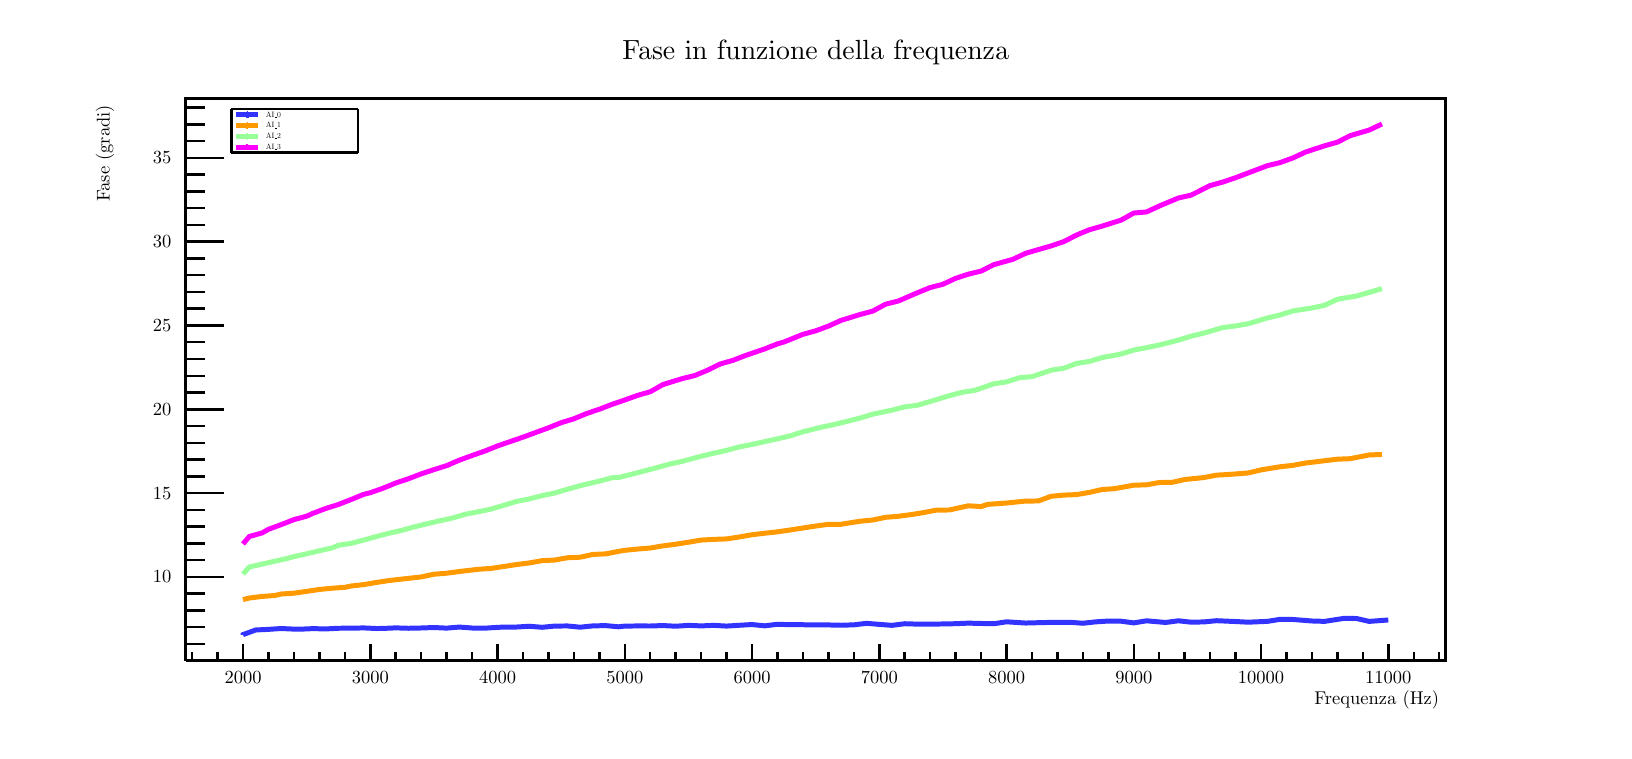
\begin{tikzpicture}
\def\CheckTikzLibraryLoaded#1{ \ifcsname tikz@library@#1@loaded\endcsname \else \PackageWarning{tikz}{usetikzlibrary{#1} is missing in the preamble.} \fi }
\CheckTikzLibraryLoaded{patterns}
\CheckTikzLibraryLoaded{plotmarks}
\pgfdeclareplotmark{cross} {
\pgfpathmoveto{\pgfpoint{-0.3\pgfplotmarksize}{\pgfplotmarksize}}
\pgfpathlineto{\pgfpoint{+0.3\pgfplotmarksize}{\pgfplotmarksize}}
\pgfpathlineto{\pgfpoint{+0.3\pgfplotmarksize}{0.3\pgfplotmarksize}}
\pgfpathlineto{\pgfpoint{+1\pgfplotmarksize}{0.3\pgfplotmarksize}}
\pgfpathlineto{\pgfpoint{+1\pgfplotmarksize}{-0.3\pgfplotmarksize}}
\pgfpathlineto{\pgfpoint{+0.3\pgfplotmarksize}{-0.3\pgfplotmarksize}}
\pgfpathlineto{\pgfpoint{+0.3\pgfplotmarksize}{-1.\pgfplotmarksize}}
\pgfpathlineto{\pgfpoint{-0.3\pgfplotmarksize}{-1.\pgfplotmarksize}}
\pgfpathlineto{\pgfpoint{-0.3\pgfplotmarksize}{-0.3\pgfplotmarksize}}
\pgfpathlineto{\pgfpoint{-1.\pgfplotmarksize}{-0.3\pgfplotmarksize}}
\pgfpathlineto{\pgfpoint{-1.\pgfplotmarksize}{0.3\pgfplotmarksize}}
\pgfpathlineto{\pgfpoint{-0.3\pgfplotmarksize}{0.3\pgfplotmarksize}}
\pgfpathclose
\pgfusepathqstroke
}
\pgfdeclareplotmark{cross*} {
\pgfpathmoveto{\pgfpoint{-0.3\pgfplotmarksize}{\pgfplotmarksize}}
\pgfpathlineto{\pgfpoint{+0.3\pgfplotmarksize}{\pgfplotmarksize}}
\pgfpathlineto{\pgfpoint{+0.3\pgfplotmarksize}{0.3\pgfplotmarksize}}
\pgfpathlineto{\pgfpoint{+1\pgfplotmarksize}{0.3\pgfplotmarksize}}
\pgfpathlineto{\pgfpoint{+1\pgfplotmarksize}{-0.3\pgfplotmarksize}}
\pgfpathlineto{\pgfpoint{+0.3\pgfplotmarksize}{-0.3\pgfplotmarksize}}
\pgfpathlineto{\pgfpoint{+0.3\pgfplotmarksize}{-1.\pgfplotmarksize}}
\pgfpathlineto{\pgfpoint{-0.3\pgfplotmarksize}{-1.\pgfplotmarksize}}
\pgfpathlineto{\pgfpoint{-0.3\pgfplotmarksize}{-0.3\pgfplotmarksize}}
\pgfpathlineto{\pgfpoint{-1.\pgfplotmarksize}{-0.3\pgfplotmarksize}}
\pgfpathlineto{\pgfpoint{-1.\pgfplotmarksize}{0.3\pgfplotmarksize}}
\pgfpathlineto{\pgfpoint{-0.3\pgfplotmarksize}{0.3\pgfplotmarksize}}
\pgfpathclose
\pgfusepathqfillstroke
}
\pgfdeclareplotmark{newstar} {
\pgfpathmoveto{\pgfqpoint{0pt}{\pgfplotmarksize}}
\pgfpathlineto{\pgfqpointpolar{44}{0.5\pgfplotmarksize}}
\pgfpathlineto{\pgfqpointpolar{18}{\pgfplotmarksize}}
\pgfpathlineto{\pgfqpointpolar{-20}{0.5\pgfplotmarksize}}
\pgfpathlineto{\pgfqpointpolar{-54}{\pgfplotmarksize}}
\pgfpathlineto{\pgfqpointpolar{-90}{0.5\pgfplotmarksize}}
\pgfpathlineto{\pgfqpointpolar{234}{\pgfplotmarksize}}
\pgfpathlineto{\pgfqpointpolar{198}{0.5\pgfplotmarksize}}
\pgfpathlineto{\pgfqpointpolar{162}{\pgfplotmarksize}}
\pgfpathlineto{\pgfqpointpolar{134}{0.5\pgfplotmarksize}}
\pgfpathclose
\pgfusepathqstroke
}
\pgfdeclareplotmark{newstar*} {
\pgfpathmoveto{\pgfqpoint{0pt}{\pgfplotmarksize}}
\pgfpathlineto{\pgfqpointpolar{44}{0.5\pgfplotmarksize}}
\pgfpathlineto{\pgfqpointpolar{18}{\pgfplotmarksize}}
\pgfpathlineto{\pgfqpointpolar{-20}{0.5\pgfplotmarksize}}
\pgfpathlineto{\pgfqpointpolar{-54}{\pgfplotmarksize}}
\pgfpathlineto{\pgfqpointpolar{-90}{0.5\pgfplotmarksize}}
\pgfpathlineto{\pgfqpointpolar{234}{\pgfplotmarksize}}
\pgfpathlineto{\pgfqpointpolar{198}{0.5\pgfplotmarksize}}
\pgfpathlineto{\pgfqpointpolar{162}{\pgfplotmarksize}}
\pgfpathlineto{\pgfqpointpolar{134}{0.5\pgfplotmarksize}}
\pgfpathclose
\pgfusepathqfillstroke
}
\definecolor{c}{rgb}{1,1,1};
\draw [color=c, fill=c] (0,0) rectangle (20,8.92231);
\draw [color=c, fill=c] (2,0.892231) rectangle (18,8.03008);
\definecolor{c}{rgb}{0,0,0};
\draw [c,line width=0.9] (2,0.892231) -- (2,8.03008) -- (18,8.03008) -- (18,0.892231) -- (2,0.892231);
\definecolor{c}{rgb}{1,1,1};
\draw [color=c, fill=c] (2,0.892231) rectangle (18,8.03008);
\definecolor{c}{rgb}{0,0,0};
\draw [c,line width=0.9] (2,0.892231) -- (2,8.03008) -- (18,8.03008) -- (18,0.892231) -- (2,0.892231);
\draw [c,line width=0.9] (2,0.892231) -- (18,0.892231);
\draw [c,line width=0.9] (2.72775,1.10637) -- (2.72775,0.892231);
\draw [c,line width=0.9] (3.05098,0.999298) -- (3.05098,0.892231);
\draw [c,line width=0.9] (3.3742,0.999298) -- (3.3742,0.892231);
\draw [c,line width=0.9] (3.69742,0.999298) -- (3.69742,0.892231);
\draw [c,line width=0.9] (4.02064,0.999298) -- (4.02064,0.892231);
\draw [c,line width=0.9] (4.34386,1.10637) -- (4.34386,0.892231);
\draw [c,line width=0.9] (4.66708,0.999298) -- (4.66708,0.892231);
\draw [c,line width=0.9] (4.9903,0.999298) -- (4.9903,0.892231);
\draw [c,line width=0.9] (5.31353,0.999298) -- (5.31353,0.892231);
\draw [c,line width=0.9] (5.63675,0.999298) -- (5.63675,0.892231);
\draw [c,line width=0.9] (5.95997,1.10637) -- (5.95997,0.892231);
\draw [c,line width=0.9] (6.28319,0.999298) -- (6.28319,0.892231);
\draw [c,line width=0.9] (6.60641,0.999298) -- (6.60641,0.892231);
\draw [c,line width=0.9] (6.92963,0.999298) -- (6.92963,0.892231);
\draw [c,line width=0.9] (7.25285,0.999298) -- (7.25285,0.892231);
\draw [c,line width=0.9] (7.57608,1.10637) -- (7.57608,0.892231);
\draw [c,line width=0.9] (7.8993,0.999298) -- (7.8993,0.892231);
\draw [c,line width=0.9] (8.22252,0.999298) -- (8.22252,0.892231);
\draw [c,line width=0.9] (8.54574,0.999298) -- (8.54574,0.892231);
\draw [c,line width=0.9] (8.86896,0.999298) -- (8.86896,0.892231);
\draw [c,line width=0.9] (9.19218,1.10637) -- (9.19218,0.892231);
\draw [c,line width=0.9] (9.5154,0.999298) -- (9.5154,0.892231);
\draw [c,line width=0.9] (9.83862,0.999298) -- (9.83862,0.892231);
\draw [c,line width=0.9] (10.1618,0.999298) -- (10.1618,0.892231);
\draw [c,line width=0.9] (10.4851,0.999298) -- (10.4851,0.892231);
\draw [c,line width=0.9] (10.8083,1.10637) -- (10.8083,0.892231);
\draw [c,line width=0.9] (11.1315,0.999298) -- (11.1315,0.892231);
\draw [c,line width=0.9] (11.4547,0.999298) -- (11.4547,0.892231);
\draw [c,line width=0.9] (11.778,0.999298) -- (11.778,0.892231);
\draw [c,line width=0.9] (12.1012,0.999298) -- (12.1012,0.892231);
\draw [c,line width=0.9] (12.4244,1.10637) -- (12.4244,0.892231);
\draw [c,line width=0.9] (12.7476,0.999298) -- (12.7476,0.892231);
\draw [c,line width=0.9] (13.0708,0.999298) -- (13.0708,0.892231);
\draw [c,line width=0.9] (13.3941,0.999298) -- (13.3941,0.892231);
\draw [c,line width=0.9] (13.7173,0.999298) -- (13.7173,0.892231);
\draw [c,line width=0.9] (14.0405,1.10637) -- (14.0405,0.892231);
\draw [c,line width=0.9] (14.3637,0.999298) -- (14.3637,0.892231);
\draw [c,line width=0.9] (14.6869,0.999298) -- (14.6869,0.892231);
\draw [c,line width=0.9] (15.0102,0.999298) -- (15.0102,0.892231);
\draw [c,line width=0.9] (15.3334,0.999298) -- (15.3334,0.892231);
\draw [c,line width=0.9] (15.6566,1.10637) -- (15.6566,0.892231);
\draw [c,line width=0.9] (15.9798,0.999298) -- (15.9798,0.892231);
\draw [c,line width=0.9] (16.3031,0.999298) -- (16.3031,0.892231);
\draw [c,line width=0.9] (16.6263,0.999298) -- (16.6263,0.892231);
\draw [c,line width=0.9] (16.9495,0.999298) -- (16.9495,0.892231);
\draw [c,line width=0.9] (17.2727,1.10637) -- (17.2727,0.892231);
\draw [c,line width=0.9] (2.72775,1.10637) -- (2.72775,0.892231);
\draw [c,line width=0.9] (2.40453,0.999298) -- (2.40453,0.892231);
\draw [c,line width=0.9] (2.08131,0.999298) -- (2.08131,0.892231);
\draw [c,line width=0.9] (17.2727,1.10637) -- (17.2727,0.892231);
\draw [c,line width=0.9] (17.5959,0.999298) -- (17.5959,0.892231);
\draw [c,line width=0.9] (17.9192,0.999298) -- (17.9192,0.892231);
\draw [anchor=base] (2.72775,0.597795) node[scale=0.667961, color=c, rotate=0]{2000};
\draw [anchor=base] (4.34386,0.597795) node[scale=0.667961, color=c, rotate=0]{3000};
\draw [anchor=base] (5.95997,0.597795) node[scale=0.667961, color=c, rotate=0]{4000};
\draw [anchor=base] (7.57608,0.597795) node[scale=0.667961, color=c, rotate=0]{5000};
\draw [anchor=base] (9.19218,0.597795) node[scale=0.667961, color=c, rotate=0]{6000};
\draw [anchor=base] (10.8083,0.597795) node[scale=0.667961, color=c, rotate=0]{7000};
\draw [anchor=base] (12.4244,0.597795) node[scale=0.667961, color=c, rotate=0]{8000};
\draw [anchor=base] (14.0405,0.597795) node[scale=0.667961, color=c, rotate=0]{9000};
\draw [anchor=base] (15.6566,0.597795) node[scale=0.667961, color=c, rotate=0]{10000};
\draw [anchor=base] (17.2727,0.597795) node[scale=0.667961, color=c, rotate=0]{11000};
\draw [anchor= east] (18,0.392582) node[scale=0.667961, color=c, rotate=0]{ Frequenza (Hz)};
\draw [c,line width=0.9] (2,0.892231) -- (2,8.03008);
\draw [c,line width=0.9] (2.48,1.95415) -- (2,1.95415);
\draw [c,line width=0.9] (2.24,2.16702) -- (2,2.16702);
\draw [c,line width=0.9] (2.24,2.37989) -- (2,2.37989);
\draw [c,line width=0.9] (2.24,2.59276) -- (2,2.59276);
\draw [c,line width=0.9] (2.24,2.80562) -- (2,2.80562);
\draw [c,line width=0.9] (2.48,3.01849) -- (2,3.01849);
\draw [c,line width=0.9] (2.24,3.23136) -- (2,3.23136);
\draw [c,line width=0.9] (2.24,3.44422) -- (2,3.44422);
\draw [c,line width=0.9] (2.24,3.65709) -- (2,3.65709);
\draw [c,line width=0.9] (2.24,3.86996) -- (2,3.86996);
\draw [c,line width=0.9] (2.48,4.08283) -- (2,4.08283);
\draw [c,line width=0.9] (2.24,4.29569) -- (2,4.29569);
\draw [c,line width=0.9] (2.24,4.50856) -- (2,4.50856);
\draw [c,line width=0.9] (2.24,4.72143) -- (2,4.72143);
\draw [c,line width=0.9] (2.24,4.9343) -- (2,4.9343);
\draw [c,line width=0.9] (2.48,5.14716) -- (2,5.14716);
\draw [c,line width=0.9] (2.24,5.36003) -- (2,5.36003);
\draw [c,line width=0.9] (2.24,5.5729) -- (2,5.5729);
\draw [c,line width=0.9] (2.24,5.78576) -- (2,5.78576);
\draw [c,line width=0.9] (2.24,5.99863) -- (2,5.99863);
\draw [c,line width=0.9] (2.48,6.2115) -- (2,6.2115);
\draw [c,line width=0.9] (2.24,6.42437) -- (2,6.42437);
\draw [c,line width=0.9] (2.24,6.63723) -- (2,6.63723);
\draw [c,line width=0.9] (2.24,6.8501) -- (2,6.8501);
\draw [c,line width=0.9] (2.24,7.06297) -- (2,7.06297);
\draw [c,line width=0.9] (2.48,7.27584) -- (2,7.27584);
\draw [c,line width=0.9] (2.48,1.95415) -- (2,1.95415);
\draw [c,line width=0.9] (2.24,1.74129) -- (2,1.74129);
\draw [c,line width=0.9] (2.24,1.52842) -- (2,1.52842);
\draw [c,line width=0.9] (2.24,1.31555) -- (2,1.31555);
\draw [c,line width=0.9] (2.24,1.10268) -- (2,1.10268);
\draw [c,line width=0.9] (2.48,7.27584) -- (2,7.27584);
\draw [c,line width=0.9] (2.24,7.4887) -- (2,7.4887);
\draw [c,line width=0.9] (2.24,7.70157) -- (2,7.70157);
\draw [c,line width=0.9] (2.24,7.91444) -- (2,7.91444);
\draw [anchor= east] (1.9,1.95415) node[scale=0.667961, color=c, rotate=0]{10};
\draw [anchor= east] (1.9,3.01849) node[scale=0.667961, color=c, rotate=0]{15};
\draw [anchor= east] (1.9,4.08283) node[scale=0.667961, color=c, rotate=0]{20};
\draw [anchor= east] (1.9,5.14716) node[scale=0.667961, color=c, rotate=0]{25};
\draw [anchor= east] (1.9,6.2115) node[scale=0.667961, color=c, rotate=0]{30};
\draw [anchor= east] (1.9,7.27584) node[scale=0.667961, color=c, rotate=0]{35};
\draw [anchor= east] (0.974186,8.03008) node[scale=0.667961, color=c, rotate=90]{ Fase (gradi)};
\definecolor{c}{rgb}{0.2,0.2,1};
\draw [c,line width=1.8] (2.72762,1.21668) -- (2.72774,1.22134) -- (2.88943,1.28008) -- (3.05092,1.28777) -- (3.21266,1.29873) -- (3.37421,1.29108) -- (3.45495,1.29009) -- (3.61662,1.29729) -- (3.7784,1.29334) -- (3.93998,1.30184) --
 (4.10157,1.30322) -- (4.26316,1.30605) -- (4.42472,1.29859) -- (4.5055,1.29951) -- (4.66716,1.30674) -- (4.82883,1.30171) -- (4.99034,1.30532) -- (5.15163,1.31136) -- (5.31349,1.30358) -- (5.47513,1.31719) -- (5.63677,1.30504) -- (5.79852,1.30292)
 -- (5.8791,1.30819) -- (6.04057,1.3173) -- (6.20219,1.31762) -- (6.364,1.32758) -- (6.52566,1.31402) -- (6.68728,1.32974) -- (6.84884,1.33099) -- (7.01031,1.3154) -- (7.17193,1.33214) -- (7.33367,1.33547) -- (7.49536,1.3205) -- (7.57626,1.32948) --
 (7.73757,1.33112) -- (7.8993,1.33059) -- (8.06097,1.33615) -- (8.22251,1.32787) -- (8.38423,1.3385) -- (8.54595,1.33201) -- (8.70764,1.33851) -- (8.86913,1.32962) -- (9.03039,1.33978) -- (9.1922,1.34896) -- (9.35379,1.33289) -- (9.51562,1.35254) --
 (9.67712,1.34725) -- (9.83873,1.34672) -- (10.0005,1.34356) -- (10.1618,1.34393) -- (10.3234,1.33998) -- (10.4851,1.34537) -- (10.6468,1.36432) -- (10.8084,1.35119) -- (10.9702,1.33882) -- (11.1318,1.35948) -- (11.2934,1.35416) -- (11.4547,1.3537)
 -- (11.6163,1.35648) -- (11.7779,1.35983) -- (11.9396,1.36693) -- (12.1013,1.36268) -- (12.2628,1.35933) -- (12.4245,1.38378) -- (12.6669,1.36816) -- (12.8284,1.37253) -- (12.9902,1.37652) -- (13.2324,1.3775) -- (13.3941,1.36542) --
 (13.5559,1.38311) -- (13.7174,1.39348) -- (13.8791,1.3914) -- (14.0404,1.37013) -- (14.202,1.39632) -- (14.4449,1.37542) -- (14.6061,1.39672) -- (14.7678,1.37927) -- (14.9295,1.38215) -- (15.091,1.39791) -- (15.3334,1.38728) -- (15.495,1.37899) --
 (15.7378,1.38935) -- (15.8989,1.41539) -- (16.0607,1.41339) -- (16.3032,1.39427) -- (16.4646,1.38938) -- (16.7073,1.42703) -- (16.8689,1.4258) -- (17.0302,1.38912) -- (17.2727,1.40713);
\definecolor{c}{rgb}{1,0.6,0};
\draw [c,line width=1.8] (2.72727,1.66576) -- (2.8085,1.68624) -- (2.97006,1.70601) -- (3.13188,1.71809) -- (3.21254,1.73667) -- (3.37423,1.74745) -- (3.53591,1.77021) -- (3.69746,1.79485) -- (3.8591,1.81047) -- (4.02066,1.8216) -- (4.1015,1.83863)
 -- (4.26324,1.85673) -- (4.42491,1.88396) -- (4.58616,1.90842) -- (4.74787,1.92676) -- (4.99043,1.95367) -- (5.15177,1.98787) -- (5.31342,2.00101) -- (5.47504,2.02264) -- (5.7179,2.05109) -- (5.87907,2.06185) -- (6.04065,2.08648) --
 (6.20256,2.11124) -- (6.36405,2.13162) -- (6.5257,2.16033) -- (6.6873,2.16853) -- (6.84883,2.19735) -- (7.01029,2.20416) -- (7.17205,2.23971) -- (7.33372,2.2464) -- (7.49527,2.27816) -- (7.57629,2.29162) -- (7.73752,2.30775) -- (7.89925,2.32106) --
 (8.06075,2.34816) -- (8.22253,2.36901) -- (8.38423,2.39469) -- (8.5456,2.42179) -- (8.70753,2.43082) -- (8.86913,2.43651) -- (9.0305,2.46118) -- (9.19224,2.48964) -- (9.35387,2.50874) -- (9.51547,2.52646) -- (9.67697,2.54996) -- (9.8387,2.57525) --
 (10.0003,2.59989) -- (10.1617,2.62217) -- (10.3234,2.62258) -- (10.5661,2.66128) -- (10.7277,2.67718) -- (10.8892,2.7109) -- (11.0508,2.72415) -- (11.2124,2.7452) -- (11.374,2.77163) -- (11.5356,2.80266) -- (11.6974,2.80392) -- (11.9396,2.85718) --
 (12.1013,2.84697) -- (12.1819,2.87507) -- (12.4247,2.8924) -- (12.6669,2.91687) -- (12.8289,2.91856) -- (12.9902,2.97794) -- (13.1518,2.99298) -- (13.3131,2.99931) -- (13.4748,3.02692) -- (13.6364,3.06377) -- (13.798,3.07513) -- (14.0406,3.11878) --
 (14.2021,3.12339) -- (14.3639,3.15273) -- (14.5254,3.1547) -- (14.6871,3.19091) -- (14.9295,3.21574) -- (15.0911,3.24649) -- (15.2527,3.25561) -- (15.4952,3.27441) -- (15.6566,3.31331) -- (15.8988,3.35287) -- (16.0606,3.37075) -- (16.2223,3.40039)
 -- (16.3838,3.41978) -- (16.6263,3.44908) -- (16.7878,3.45536) -- (17.0301,3.50291) -- (17.192,3.50879);
\definecolor{c}{rgb}{0.6,1,0.6};
\draw [c,line width=1.8] (2.72751,1.99085) -- (2.80843,2.07992) -- (2.9702,2.11678) -- (3.13192,2.15324) -- (3.29322,2.1894) -- (3.37422,2.21182) -- (3.53601,2.24751) -- (3.69753,2.28564) -- (3.85937,2.32248) -- (3.93965,2.35657) -- (4.10172,2.38005)
 -- (4.26328,2.42279) -- (4.42488,2.46762) -- (4.58619,2.50977) -- (4.74788,2.54636) -- (4.90945,2.59146) -- (5.071,2.63037) -- (5.23279,2.66782) -- (5.39444,2.70356) -- (5.55601,2.75115) -- (5.71781,2.78153) -- (5.87915,2.81633) -- (6.04077,2.86334)
 -- (6.20228,2.91288) -- (6.36404,2.94472) -- (6.52566,2.98569) -- (6.68739,3.01999) -- (6.84886,3.06751) -- (7.01027,3.1131) -- (7.25301,3.17058) -- (7.41463,3.21351) -- (7.4952,3.21559) -- (7.65687,3.25592) -- (7.81875,3.29878) -- (7.9802,3.34079)
 -- (8.14184,3.38592) -- (8.30317,3.42133) -- (8.54599,3.48675) -- (8.70759,3.52516) -- (8.86924,3.56156) -- (9.03055,3.60492) -- (9.19219,3.63624) -- (9.35367,3.67255) -- (9.51545,3.70799) -- (9.6771,3.74465) -- (9.83872,3.79744) --
 (10.0811,3.85716) -- (10.2427,3.89078) -- (10.4043,3.93061) -- (10.5661,3.97205) -- (10.7274,4.0213) -- (10.9699,4.07207) -- (11.1317,4.11335) -- (11.2935,4.13452) -- (11.4547,4.18167) -- (11.6973,4.25517) -- (11.8588,4.29823) -- (12.0203,4.32321)
 -- (12.2629,4.40628) -- (12.4246,4.43083) -- (12.5862,4.48292) -- (12.7478,4.49766) -- (12.9903,4.57947) -- (13.1521,4.60426) -- (13.313,4.66478) -- (13.4749,4.69055) -- (13.6365,4.73918) -- (13.8791,4.78515) -- (14.0402,4.83522) --
 (14.2022,4.86512) -- (14.3638,4.89914) -- (14.606,4.96105) -- (14.7678,5.01118) -- (14.9294,5.05028) -- (15.1718,5.12091) -- (15.3334,5.14137) -- (15.495,5.17) -- (15.7374,5.24246) -- (15.8992,5.28069) -- (16.0607,5.33147) -- (16.3034,5.36943) --
 (16.4646,5.40405) -- (16.6263,5.48017) -- (16.869,5.52126) -- (17.0304,5.56721) -- (17.1918,5.61559);
\definecolor{c}{rgb}{1,0,1};
\draw [c,line width=1.8] (2.7276,2.37328) -- (2.80853,2.46727) -- (2.97017,2.51266) -- (3.05074,2.55848) -- (3.21247,2.61807) -- (3.37422,2.68145) -- (3.53596,2.72494) -- (3.61655,2.7619) -- (3.77818,2.82309) -- (3.94,2.87379) -- (4.10157,2.93736) --
 (4.26315,3.0032) -- (4.34394,3.02292) -- (4.50563,3.08007) -- (4.66715,3.14652) -- (4.82875,3.20067) -- (4.9904,3.26229) -- (5.15183,3.31643) -- (5.3135,3.36689) -- (5.47514,3.43709) -- (5.63684,3.49565) -- (5.79836,3.55227) -- (5.95996,3.61765) --
 (6.12172,3.67311) -- (6.28343,3.72875) -- (6.44461,3.78792) -- (6.60636,3.84766) -- (6.768,3.91236) -- (6.92967,3.96219) -- (7.09133,4.02913) -- (7.25297,4.08324) -- (7.4146,4.14575) -- (7.57627,4.20071) -- (7.73763,4.25899) -- (7.89931,4.30541) --
 (8.06076,4.39682) -- (8.30323,4.47175) -- (8.46499,4.51147) -- (8.62663,4.57866) -- (8.7883,4.65805) -- (8.94968,4.70448) -- (9.11152,4.76655) -- (9.35382,4.84991) -- (9.51551,4.91359) -- (9.596,4.93657) -- (9.8388,5.03507) -- (10.0004,5.07918) --
 (10.1618,5.13894) -- (10.3235,5.21226) -- (10.5661,5.2872) -- (10.7278,5.33025) -- (10.8889,5.41777) -- (11.0508,5.45803) -- (11.2934,5.56301) -- (11.4546,5.62896) -- (11.6162,5.67045) -- (11.7779,5.74606) -- (11.9397,5.79869) -- (12.1013,5.83823)
 -- (12.2629,5.9195) -- (12.5052,5.98755) -- (12.6669,6.06356) -- (12.8283,6.11122) -- (12.9901,6.15737) -- (13.1519,6.21211) -- (13.3132,6.29523) -- (13.4748,6.3625) -- (13.6364,6.40876) -- (13.8791,6.48506) -- (14.0405,6.57516) -- (14.2023,6.5891)
 -- (14.3637,6.66401) -- (14.6061,6.76595) -- (14.7678,6.80228) -- (15.0103,6.92426) -- (15.1718,6.96895) -- (15.3335,7.02393) -- (15.576,7.11566) -- (15.7376,7.1766) -- (15.8991,7.21613) -- (16.0607,7.27473) -- (16.2222,7.34972) -- (16.4647,7.42952)
 -- (16.6262,7.47496) -- (16.7879,7.55732) -- (17.03,7.62933) -- (17.1918,7.70563);
\definecolor{c}{rgb}{1,1,1};
\draw [color=c, fill=c] (2.58145,7.34336) rectangle (4.18546,7.89474);
\definecolor{c}{rgb}{0,0,0};
\draw [c,line width=0.9] (2.58145,7.34336) -- (4.18546,7.34336);
\draw [c,line width=0.9] (4.18546,7.34336) -- (4.18546,7.89474);
\draw [c,line width=0.9] (4.18546,7.89474) -- (2.58145,7.89474);
\draw [c,line width=0.9] (2.58145,7.89474) -- (2.58145,7.34336);
\draw [anchor=base west] (2.98246,7.7948) node[scale=0.278317, color=c, rotate=0]{AI\_0};
\definecolor{c}{rgb}{1,1,1};
\draw [c, fill=c] (2.6416,7.77757) -- (2.92231,7.77757) -- (2.92231,7.87406) -- (2.6416,7.87406);
\definecolor{c}{rgb}{0.2,0.2,1};
\draw [c,line width=1.8] (2.6416,7.82582) -- (2.92231,7.82582);
\foreach \P in {(2.78196,7.82582)}{\draw[mark options={color=c,fill=c},mark size=2.402402pt, line width=0.000000pt, mark=*,mark size=1pt] plot coordinates {\P};}
\definecolor{c}{rgb}{0,0,0};
\draw [anchor=base west] (2.98246,7.65696) node[scale=0.278317, color=c, rotate=0]{AI\_1};
\definecolor{c}{rgb}{1,1,1};
\draw [c, fill=c] (2.6416,7.63972) -- (2.92231,7.63972) -- (2.92231,7.73622) -- (2.6416,7.73622);
\definecolor{c}{rgb}{1,0.6,0};
\draw [c,line width=1.8] (2.6416,7.68797) -- (2.92231,7.68797);
\foreach \P in {(2.78196,7.68797)}{\draw[mark options={color=c,fill=c},mark size=2.402402pt, line width=0.000000pt, mark=*,mark size=1pt] plot coordinates {\P};}
\definecolor{c}{rgb}{0,0,0};
\draw [anchor=base west] (2.98246,7.51911) node[scale=0.278317, color=c, rotate=0]{AI\_2};
\definecolor{c}{rgb}{1,1,1};
\draw [c, fill=c] (2.6416,7.50188) -- (2.92231,7.50188) -- (2.92231,7.59837) -- (2.6416,7.59837);
\definecolor{c}{rgb}{0.6,1,0.6};
\draw [c,line width=1.8] (2.6416,7.55013) -- (2.92231,7.55013);
\foreach \P in {(2.78196,7.55013)}{\draw[mark options={color=c,fill=c},mark size=2.402402pt, line width=0.000000pt, mark=*,mark size=1pt] plot coordinates {\P};}
\definecolor{c}{rgb}{0,0,0};
\draw [anchor=base west] (2.98246,7.38127) node[scale=0.278317, color=c, rotate=0]{AI\_3};
\definecolor{c}{rgb}{1,1,1};
\draw [c, fill=c] (2.6416,7.36404) -- (2.92231,7.36404) -- (2.92231,7.46053) -- (2.6416,7.46053);
\definecolor{c}{rgb}{1,0,1};
\draw [c,line width=1.8] (2.6416,7.41228) -- (2.92231,7.41228);
\foreach \P in {(2.78196,7.41228)}{\draw[mark options={color=c,fill=c},mark size=2.402402pt, line width=0.000000pt, mark=*,mark size=1pt] plot coordinates {\P};}
\definecolor{c}{rgb}{0,0,0};
\draw (10,8.60702) node[scale=1.00194, color=c, rotate=0]{Fase in funzione della frequenza};
\end{tikzpicture}
%\end{document}
